\documentclass[a4paper,12pt]{article}

\usepackage{pgfplots}
\pgfplotsset{compat=1.18}
\pgfplotsset{compat/show suggested version=false}

\usepackage{siunitx}
\sisetup{locale=DE}

\pagestyle{empty}

\begin{document}
\begin{center}
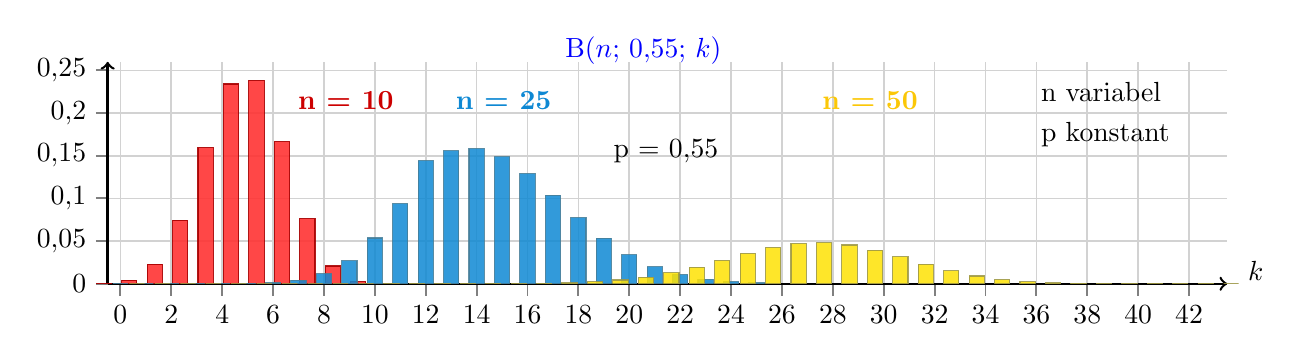
\begin{tikzpicture}
\begin{axis}[
  width=15.8cm,
  height=4.4cm,
  ybar,
  bar width=5.5pt,
  enlarge x limits={abs=0.8},
  xmin=-0.5, xmax=43.5,          % <- bis 43 abgeschnitten (mit Rand)
  ymin=0, ymax=0.26,
  axis lines=left,
  axis line style={->, line width=0.9pt},
  tick align=outside,
  tick style={line width=0.7pt},
  xtick={0,2,...,42},            % <- letzte gerade Zahl im Bereich
  ytick={0,0.05,...,0.25},
  yticklabel style={
    /pgf/number format/fixed,
    /pgf/number format/precision=2,
    /pgf/number format/use comma
  },
  grid=major,
  grid style={gray!35, line width=0.6pt},
  clip=false
]

% --- Rot: n=10 (links) ---
\addplot+[
  bar shift=-6pt,
  fill=red!80,
  draw=red!65!black,
  line width=0.4pt,
  opacity=0.90
] coordinates {
(0,3.405062891602e-04) (1,4.161743534180e-03) (2,2.288958943799e-02)
(3,7.460310631641e-02) (4,1.595677551768e-01) (5,2.340327075926e-01)
(6,2.383666466221e-01) (7,1.664782928789e-01) (8,7.630255090287e-02)
(9,2.073839288667e-02) (10,2.533130864807e-03)
};

% --- Blau: n=25 (mitte) ---
\addplot+[
  bar shift=0pt,
  fill=cyan!70!blue,
  draw=cyan!55!black,
  line width=0.4pt,
  opacity=0.85
] coordinates {
(0,2.139502727067e-09) (1,6.537369443816e-08) (2,9.588141850930e-07)
(3,8.984444030686e-06) (4,6.039542931739e-05) (5,3.100298704959e-04)
(6,1.263084657576e-03) (7,4.190233229102e-03) (8,1.152314138006e-02)
(9,2.679109158213e-02) (10,5.363061978689e-02) (11,9.385358452706e-02)
(12,1.443278114166e-01) (13,1.556666446329e-01) (14,1.583058314819e-01)
(15,1.486833168391e-01) (16,1.291322265485e-01) (17,1.037885036175e-01)
(18,7.737292251874e-02) (19,5.332604071422e-02) (20,3.392111682760e-02)
(21,1.989544725336e-02) (22,1.071298565905e-02) (23,5.268563930338e-03)
(24,2.327492408795e-03) (25,9.030732935249e-04)
};

% --- Gelb: n=50 (rechts) --- 0..43
\addplot+[
  bar shift=+6pt,
  fill=yellow!85!orange,
  draw=yellow!55!black,
  line width=0.4pt,
  opacity=0.85
] coordinates {
(0,4.577471919127e-18) (1,2.797343950578e-16) (2,8.376491052008e-15)
(3,1.638069361282e-13) (4,2.352449610507e-12) (5,2.645198895370e-11)
(6,2.424765654089e-10) (7,1.862835835840e-09) (8,1.223779653266e-08)
(9,6.957704488573e-08) (10,3.457455229566e-07) (11,1.512097737294e-06)
(12,5.888739044035e-06) (13,2.050145894573e-05) (14,6.412956415267e-05)
(15,1.810861503205e-04) (16,4.626793529058e-04) (17,1.073910878399e-03)
(18,2.271048246375e-03) (19,4.398739101699e-03) (20,7.830287955527e-03)
(21,1.284362607477e-02) (22,1.945572778681e-02) (23,2.731558614495e-02)
(24,3.552606519526e-02) (25,4.264569668514e-02) (26,4.707618577724e-02)
(27,4.818435257137e-02) (28,4.542397744353e-02) (29,3.944961173520e-02)
(30,3.145575126674e-02) (31,2.292890609299e-02) (32,1.520479883054e-02)
(33,9.106127079757e-03) (34,4.872997754300e-03) (35,2.317316433465e-03)
(36,9.699947136467e-04) (37,3.521674544089e-04) (38,1.088928391264e-04)
(39,2.803555173398e-05) (40,5.830407006133e-06) (41,9.504771420140e-07)
(42,1.173267994881e-07) (43,1.032423762219e-08)
};

% Beschriftungen
\node[anchor=west] at (rel axis cs:0.4,1.05) {\textcolor{blue}{$\mathrm{B}(n;\,0{,}55;\,k)$}};

\node[anchor=west, text=red!80!black, font=\bfseries] at (axis cs:6.6,0.215) {n = 10};
\node[anchor=west, text=cyan!70!blue, font=\bfseries] at (axis cs:12.8,0.215) {n = 25};
\node[anchor=west, text=yellow!60!orange, font=\bfseries] at (axis cs:27.2,0.215) {n = 50};

\node[anchor=west] at (axis cs:19.0,0.155) {p = 0,55};

\node[anchor=west] at (axis cs:35.8,0.225) {n variabel};
\node[anchor=west] at (axis cs:35.8,0.175) {p konstant};

\node[anchor=west] at (rel axis cs:1.01,0.06) {$k$};

\end{axis}
\end{tikzpicture}
\end{center}
\end{document}